\chapter{Bitcoin core}
\label{chap:bitcoin core}

\section{Introduzione}\label{sec:introduzionebitcoincore}

Bitcoin core è il successore della versione rilasciata da Satoshi Nakamoto ora conosciuta come “satoshi client”; attualmente è il client di riferimento del protocollo Bitcoin.
Bitcoin core è un progetto open-source scritto in C++, il cui codice sorgente risiede attualmente su Github sotto licenza MIT e viene sviluppato da una comunità aperta di volontari; esso costituisce una riscrittura quasi completa della versione 0.1.0 del client rilasciato da Satoshi Nakamoto.

\section{Blocchi}
\label{sec:blocchibitcoincore}

Così come le transazioni, il blocco viene definito attraverso una struttura dati: una volta creato e pubblicato un blocco, viene serializzato all’interno di un flat file, mantenendo i riferimenti necessari per eseguire la deserializzazione all’interno del database LevelDB di Google; le informazioni necessarie del blocco vengono contenute all’interno una struttura chiamata BlockHeader e la dimensione della struttura da deserializzare è pari a 80 byte, come rappresentato in Tabella \ref{tab:blockheaderbitcoinc}

\begin{table}
       \centering\small
           \begin{tabular}{|c|c|}
               \hline
                 \multicolumn{2}{|c|}{\textbf{BlockHeader}} \\
                 %\cmidrule(lr){1-2}
                 \hline
                 \multicolumn{1}{|c|}{Type} & \multicolumn{1}{c|}{Name} \\
               \hline \hline
               $int32\_t$ & nVersion   \\
               \hline
               $uint256$ & hashPrevBlock \\
                \hline
               $uint256$ & hashMerkleRoot \\
                \hline
               $uint32\_t$ & nTime \\
                \hline
               $uint32\_t$ & nBits \\
                \hline
               $uint32\_t$ & nNonce \\
               \hline
       \end{tabular}
       \caption{Struttura di un block header in Bitcoin core.\label{tab:blockheaderbitcoinc}}
   \end{table}


\begin{itemize}
  \item {\bf nVersion\/}: Identifica le regole seguite dal blocco; fino ad ora si possono identificare 4 versioni, tutte introdotte attraverso dei soft-fork.
  \item {\bf hashPrevBlock e hashMerkleRoot\/}: Appartengono ad un tipo di dato non primitivo del C++, ma ad un tipo definito da Bitcoin core. Rappresentano una struttura dati da 32 byte in cui vengono memorizzati l’hash del blocco precedente (in {\tt{hashPrevBlock}}) e la radice del Merkle Tree (in {\tt{hashMerkleRoot}}); queste ultime garantiscono che il blocco non possa in nessun modo essere modificato, senza alterare l’intestazione del blocco.
  \item {\bf nTime\/}: Valore che rappresenta un’epoca Unix e indica il momento in cui il miner ha iniziato ad eseguire la Proof of Work per convalidare il blocco.
  \item {\bf nBits\/}: Un intero a 8 byte, che rappresenta il target di difficoltà dell’algoritmo di PoW del blocco.
  \item {\bf nNonce\/}: Valore intero a 8 byte usato per contenere il valore generato dall’algoritmo di PoW.
\end{itemize}

Il blocco, oltre a contenere l’intestazione, contiene ulteriori informazioni riguardo la sua dimensione e la rete di appartenenza: infatti il client Bitcoin può essere eseguito anche in modalità testnet, in cui vengono testate le nuove versioni del software prima del rilascio ufficiale.
La struttura finale del blocco, nella version attuale, può essere rappresentata nel modo indicato in Tabella \ref{tab:blockbitcoinc}

\begin{table}
       \centering\small
           \begin{tabular}{|c|c|}
               \hline
                 \multicolumn{2}{|c|}{\textbf{Block}} \\
                 %\cmidrule(lr){1-2}
                 \hline
                 \multicolumn{1}{|c|}{Type} & \multicolumn{1}{c|}{Name} \\
               \hline \hline
               $int32\_t$ & magicNumber   \\
               \hline
               $int32\_t$ & blockSize \\
               \hline
               BlockHeader & blockHeader \\
               \hline
               CompactSize & numberTx \\
               \hline
               vector<RawTransaction> & transactions \\
               \hline
       \end{tabular}
       \caption{Struttura di un blocco in Bitcoin core.\label{tab:blockbitcoinc}}
   \end{table}

\begin{itemize}
  \setlength\itemsep{1em}
  \item {\bf magicNumber\/}: Rappresenta una signature per la struttura dati e non è qualcosa di specifico per Bitcoin; il numero magico viene usato, infatti, nell’informatica per i file e i protocolli, per semplificare notevolmente il riconoscimento del file o della struttura dati: ad esempio il numero magico per un file png è 89504E470D0A1A0A, mentre il numero magico di bitcoin per la rete principale è rappresentato da 0xD9B4BEF9.
  \item {\bf numberTx\/}: Il valore rappresenta il numero di transazioni contenute all'interno del blocco e viene serializzato usando un metodo simile alla tecnica di memorizzazione dei record a lunghezza variabile all’interno di un database relazionale; in Bitcoin core viene rappresentato attraverso un tipo di dato che porta il nome di VarInt (intero variabile) e questo valore occupa da 1 a 9 byte di spazio.
  Il client utilizza VarInt all’interno di LevelDB, ma utilizza il tipo di dato CompactSize rilasciato nella versione 0.1.0 di Satoshi per la serializzazione all’interno del file.
\end{itemize}

\section{Transazioni}
\label{sec:transazionibitcoincore}
Come descritto nel Capitolo di \ref{sec:transazioniBitcoin}, esse rappresentano l’elemento fulcro del sistema; nel corso degli anni, gli sviluppatori di Bitcoin core hanno dovuto confrontarsi con problemi nell’implementazione originale delle transazioni: uno di essi è conosciuto come problema di malleabilità.
La malleabilità di una transizione consisteva nella possibilità di alterare l’identificativo della transizione (txId) durante il processo di verifica senza invalidarla. La motivazione dell’alterazione era dovuta alla possibilità di modificare le firme nello script di sblocco (scriptSig) senza cambiare il loro significato; quindi per il modo in cui viene calcolato l’hash della transizione, questa alterazione comportava inevitabilmente l’alterazione dell’hash, portando all’interno del protocollo le seguenti problematiche:
\begin{itemize}
  \item Il mittente non può più riconoscere la sua transazione dopo che essa è stata modificata.
  \item Le transazioni modificate sono effettivamente riconosciute come doppie spese, perché il mittente, non riuscendo più a riconoscere la sua transazione di input creata in precedenza, si ritroverà i bitcoin invariati e potrà spenderli una seconda volta.
  Questo problema non grava sul mittente, ma sull’intero sistema Bitcoin: ad esempio le transazioni che non vengono riconosciute dal mittente saranno sepolte all’interno della blockchain perché mai nessuno sarà in grado di spenderle.
\end{itemize}

Nel 2016 la community arrivò ad una soluzione tramite un soft-fork, che introdusse notevoli cambiamenti strutturali, risolvendo tutti i problemi relativi alla malleabilità di una transazione. Questo aggiornamento venne chiamato \say{Segregated Witness} e suddivise le transazioni in diverse parti, che possono essere gestite separatamente, sostituì le firme digitali con un segnaposto all’interno delle transazioni spostando le vere firme in una struttura dati differente. Questa soluzione non esclude però la possibilità che una transazione non sia malleabile, ma esclude una modifica dell’hash durante la verifica, poiché i dati utilizzati per il calcolo sono contenuti all’interno di uno spazio protetto; da qui nasce il nome Segregated Witness.

La struttura riportata in Figura \ref{tab:rawtxbitcoinc} rappresenta la struttura delle transazioni:

\begin{table}
       \centering\small
           \begin{tabular}{|c|c|}
               \hline
                 \multicolumn{2}{|c|}{\textbf{RawTransaction}} \\
                 %\cmidrule(lr){1-2}
                 \hline
                 \multicolumn{1}{|c|}{Type} & \multicolumn{1}{c|}{Name} \\
               \hline \hline
               $int32\_t$ & version   \\
               \hline
               $uint8\_t$ & marker \\
               \hline
               $uint8\_t$ & flag \\
               \hline
               CompactSize & numberTxIn \\
               \hline
               vector<TransactionInput> & transactionsInput \\
               \hline
               CompactSize & numberTxOut \\
               \hline
               vector<TransactionOutput> & transactionsOutput \\
               \hline
               vector<TransactionWitness> & transactionsWitness \\
               \hline
       \end{tabular}
       \caption{Struttura della transazione dopo l’aggiornamento al Segregated witness.\label{tab:rawtxbitcoinc}}
   \end{table}

\begin{itemize}
  \item {\bf marker e flag\/}: Sono valori interi a 1 byte che fungono da identificativo per una transazione conforme al formato Segregated Witness (SegWit); per i wallet non conformi al SegWit la transazione risulterà non valida, perché identifica una transazione con 0 input e 1 output.
  \item {\bf transactionsWitness\/}: Questa lista non è preceduta da una dimensione perché la singola transazione witness ha senso solo se esiste un input correlato, quindi la dimensione di questa lista è uguale alla dimensione della lista delle transazioni di input.
\end{itemize}

Le transazioni di input sono definite tramite una struttura rappresentata dalla Tabella \ref{tab:inputtxbitcoinc}.

\begin{table}
       \centering\small
           \begin{tabular}{|c|c|}
               \hline
                 \multicolumn{2}{|c|}{\textbf{TransactionInput}} \\
                % \cmidrule(lr){1-2}
                \hline \hline
                 \multicolumn{1}{|c|}{Type} & \multicolumn{1}{c|}{Name} \\
               \hline
               Outpoint & outpoint   \\
               \hline
               CScript & scriptSig \\
               \hline
               $uint32\_t$ & nSequence \\
               \hline
       \end{tabular}
       \caption{La struttura della transazione input all’interno di Bitcoin core.\label{tab:inputtxbitcoinc}}
   \end{table}

\begin{itemize}
  \item {\bf nSequence\/}:  Il valore viene utilizzato per esprimere il timelock relativo a livello di transazione (argomento trattato nel Capitolo \ref{sec:bitcoinScriptBitcoinCore}).
  \item {\bf scriptSig\/}: Rappresenta la condizione di sblocco espressa dalla transazione sotto forma di script.
\end{itemize}

Il tipo di dato Outpoint utilizzato nella transazione di input contiene le informazioni necessarie per identificare la transazione di output contenuta in una transazione precedente. La Tabella \ref{tab:outpointbitcoinc} ne descrive la struttura.


\begin{table}
       \centering\small
           \begin{tabular}{|c|c|}
               \hline
                 \multicolumn{2}{|c|}{\textbf{Outpoint}} \\
                % \cmidrule(lr){1-2}
                \hline \hline
                 \multicolumn{1}{|c|}{Type} & \multicolumn{1}{c|}{Name} \\
               \hline
               $uint256$ & hash   \\
               \hline
               $uint32\_t$ & index \\
              \hline
       \end{tabular}
       \caption{Struttura del tipo di dato Outpoint di Bitcoin core.\label{tab:outpointbitcoinc}}
   \end{table}

\begin{itemize}
  \item {\bf hash\/}:  Rappresenta l’hash delle transazione precedente che contiene l’UTXO sbloccato dalla transazione di input che contiene outpoint.
  \item {\bf index\/}: Il valore indica l’indice della lista in cui è memorizzato l’UTXO nella transazione precedente.
\end{itemize}

La struttura della transazione di output contiene esclusivamente le informazione dello script di blocco e il valore di bitcoin (in satoshi); in Tabella \ref{tab:transactionOutput} viene illustrata la struttura dati corrispondente.

\begin{table}[H]
       \centering\small
           \begin{tabular}{|c|c|}
               \hline
                 \multicolumn{2}{|c|}{\textbf{TransactionOutput}} \\
                % \cmidrule(lr){1-2}
                \hline \hline
                 \multicolumn{1}{|c|}{Type} & \multicolumn{1}{c|}{Name} \\
               \hline
               $int64\_t$ & nValue   \\
               \hline
               CScript & scriptPubKey \\
               \hline
       \end{tabular}
       \caption{La struttura della transazione di output di Bitcoin core.\label{tab:transactionOutput}}
   \end{table}

\begin{itemize}
  \item {\bf nValue\/}: Rappresenta il valore di bitcoin (in satoshi) contenuti nella transazione.
  \item {\bf scriptPubKey\/}: Rappresenta la condizione di blocco espressa dalla transazione sotto forma di script.
\end{itemize}

La transazione Witness rappresenta la serializzazione di tutti i dati del testimone; in Tabella \ref{tab:witnesstxbitcoinc} viene illustrata la  struttura dati corrispondente.

\begin{table}[H]
       \centering\small
           \begin{tabular}{|c|c|}
               \hline
                 \multicolumn{2}{|c|}{\textbf{TransactionWitness}} \\
                 %\cmidrule(lr){1-2}
                 \hline
                 \multicolumn{1}{|c|}{Type} & \multicolumn{1}{c|}{Name} \\
               \hline \hline
               CompactSize & stackSize   \\
               \hline
               CScript & stack \\
               \hline
       \end{tabular}
       \caption{La struttura della serializzazione dei dati del testimone; in Bitcoin core questa struttura è chiamata CScriptWitness.\label{tab:witnesstxbitcoinc}}
   \end{table}

\begin{itemize}
  \item {\bf stackSize\/}: Il valore rappresenta il numero di script contenuti all’interno della transazione.
  \item {\bf stack\/}: Il valore contiene la lista di script per la singola transazione di input.
\end{itemize}
\leavevmode
\newline
Il tipo di dato CScript è un tipo di dato contenente le informazioni necessarie per lo script; la Tabella \ref{tab:scriptbitcoinc} ne descrive la struttura.


\begin{table}
       \centering\small
           \begin{tabular}{|c|c|}
               \hline
                 \multicolumn{2}{|c|}{\textbf{CScript}} \\
                 %\cmidrule(lr){1-2}
                 \hline
                 \multicolumn{1}{|c|}{Type} & \multicolumn{1}{c|}{Name} \\
               \hline \hline
               CompactSize & scriptSize   \\
               \hline
               vector<unsigned char> & script \\
               \hline
       \end{tabular}
       \caption{Struttura del tipi di dato CScript di Bitcoin core.\label{tab:scriptbitcoinc}}
   \end{table}

\begin{itemize}
  \item {\bf scriptSize\/}: Rappresenta la lunghezza in byte dello script, espressa tramite il tipo di dato CompactSize.
  \item {\bf script\/}: Rappresenta il vettore di byte dello script.
\end{itemize}
\leavevmode
%\newpage
\section{Bitcoin script}
\label{sec:bitcoinScriptBitcoinCore}

L’aggiornamento Segregated Witness comporta un notevole cambiamento anche sulla modalità di spesa degli UTXO; infatti tutti i tipi di transazione visti finora fanno riferimento allo script di sblocco, contenuto all’interno della transazione di input.
Con il nuovo aggiornamento lo script di sblocco viene spostato all’interno di una struttura al di fuori delle transazioni di input, chiamata \say{Transazione Witness} e mostrata in Tabella \ref{tab:rawtxbitcoinc}.
I dati relativi alle transazioni witness non contengono le informazioni di una reale transazione, bensì costituiscono uno spazio riservato per esprimere la condizione di sblocco.
Per sbloccare un UTXO con il Segregated Witness bisogna far riferimento allo script contenuto all’interno delle transazioni witness, come illustrato in Tabella \ref{tab:witnesstxbitcoinc} (che chiameremo script witness). Questa modifica nella spesa degli UTXO ha costretto Bitcoin script ad un soft fork: ogni script d’ora in poi conterrà un numero di versione all’inizio che permette l’identificazione del tipo di transazione; lo script inizierà con un numero di versione uguale a zero per identificare uno script Witness, rendendo la transazione interpretabile anche da wallet non abilitati al Segregated Witness. Attraverso questa soluzione la transazione risulta essere spendibile da chiunque.
Gli script P2PKH e P2SH con il testimone segregato si evolvono in P2WPKH e P2WSH

\subsection{P2WPKH}

Lo script {\it pay-to-witness-public-key-hash \/} si semplifica notevolmente rispetto allo script P2PKH: infatti lo script witness include la versione di verifica e l’hash della chiave pubblica come nello script  P2PKH,  ma in P2WPKH è chiamato “programma di controllo”, composto da 20 byte.

Un esempio generalizzato:
\begin{lstlisting}[language=bitcoinscript, label={code:generalexamplep2wpkh}, caption={Esempio generale della struttura di uno script P2WPKH.}]
<versione di controllo> <programma di controllo>
\end{lstlisting}

Un esempio reale:
\begin{lstlisting}[language=bitcoinscript, label={code:xamplep2wpkh}, caption={Esempio reale di uno script P2WPKH.}]
0 ab68025513c3dbd2f7b92a94e0581f5d50f654e7
\end{lstlisting}

\subsection{P2WSH}

Lo script \emph{pay-to-witness-script-hash}, come lo script P2WPKH, semplifica notevolmente il predecessore e lo sostituisce interamente; un esempio di script P2WSH può essere il seguente:
\begin{lstlisting}[language=bitcoinscript, label={code:examplep2wsh}, caption={Esempio di uno script P2WSH.}]
0 a9b7b38d972cabc7961dbfbcb841ad4508d133c47ba87457b4a0e8aae86dbb89
\end{lstlisting}
Esso è molto simile allo script P2WPKH, ma con l’unica differenza della dimensione del programma di controllo impostata a 32 byte; la dimensione del programma di controllo è l’unico modo per differenziare le due tipologie di script.
La coesistenza delle transazioni tradizionali e delle transazioni con testimone segregato introduce  un problema nella comunicazione tra wallet con versioni differenti, il quale è risolto dalla possibilità di costruire un indirizzo P2SH a partire da uno script witness; inoltre, come per gli script P2SH, è possibile codificare lo script witness in un indirizzo bitcoin utilizzando una codifica Base32 con checksum, rispetto alla codifica Base58 per gli indirizzi Bitcoin tradizionali; quest’ultimo sarà simile ai seguenti indirizzi.

Per la rete Mainet:
\begin{lstlisting}[language=bitcoinscript, label={code:examplep2wsh}, caption={Address base32 della rete mainet.}]
bc1qs0c2eqayqq7afzgy38u48ytwgkkvy8yae7uu6r
\end{lstlisting}
Per la rete Testnet:
\begin{lstlisting}[language=bitcoinscript, label={code:examplep2wsh}, caption={Address base32 della rete testnet.}]
tb1qknj2fafudjfaa9nesf7rypc0hu38p04yp5ks6g
\end{lstlisting}
Questi nuovi indirizzi vengono utilizzati estensivamente dalle tecnologie Lightning network; inoltre, essi introducono notevoli benefici per le funzioni del Bitcoin.

\subsection{Transazioni non standard}
Definire solo sette tipi di script tramite Bitcoin script potrebbe risultare restrittivo; infatti negli anni il linguaggio ha subito notevoli evoluzioni grazie alle quali si possono ottenere script complessi che eseguono operazioni non banali. Queste evoluzioni hanno sopratutto reso possibile lo sviluppo di tecnologie che lavorano a stretto contatto con la tecnologia Bitcoin e che puntano a migliorare le parti del protocollo che rendono Bitcoin inadatto per alcune applicazioni del mondo reale. Ad esempio, la velocità delle transazione risulta essere un punto debole di Bitcoin a causa dell’algoritmo di PoW; questo limite viene aggirato con la proposta di un layer addizionale, conosciuto come Lightning Network, il quale usa una caratteristica di Bitcoin script conosciuta come timelock relativo (introdotto nel Paragrafo \ref{sec:relativetimelock}) con cui si può utilizzare Bitcoin offchain.

In Figura \ref{fig:velocitytx} viene illustrato il confronto delle transazioni per secondo (tps) tra Bitcoin e la tecnologia Lightning Network.

{\centering
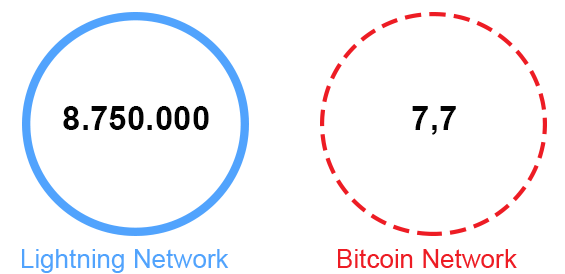
\includegraphics[scale=0.35]{images/Lightning-Network-study.png}
\captionof{figure}{Confronto tra le tecnologie Lightning network e Bitcoin: transazioni per secondo (tps)  \cite{satalight:lightningstudy}.\label{fig:velocitytx}}
\par}

\subsubsection{Timelock}

I timelock vengono introdotti nel 2016 e sono usati per esprimere restrizioni sulla modalità di spesa di UTXO al fine di consentire lo sblocco di questi ultimi solo dopo un certo evento. Questa definizione non è nuova nella tecnologia Bitcoin perché con il campo {\tt{nLockTime}} della transazione è possibile esprimere una restrizione sulla modalità di spesa di una transazione (argomento trattato nel Capitolo \ref{sec:transazioniBitcoin}); questo tipo di restrizione soffre di un problema illustrato nel seguente esempio (tratto dal libro \cite{bitcoinbook}).

\begin{example}

Supponiamo che Alice firmi una transazione spedendo uno dei suoi UTXO all'indirizzo di Bob impostando la transazione con un nLocktime proiettato nel futuro di 3 mesi.
Con questa transazione Alice e Bob sanno che:
\begin{itemize}
  \item Bob non può trasmettere la transazione per riscattare i fondi fino a quando non sono trascorsi 3 mesi.
  \item Bob può trasmettere la transazione dopo 3 mesi.
\end{itemize}
Però:
\begin{itemize}
  \item Alice può creare un'altra transazione, spendendo due volte gli stessi input senza un locktime. Pertanto, Alice può spendere lo stesso UTXO prima che siano trascorsi i 3 mesi.
  \item Bob non ha alcuna garanzia che Alice non lo farà.
\end{itemize}
\end{example}

Il concetto di timelock introduce un nuovo operatore in Bitcoin Script che prende il nome di OP\_CHECKLOCKTIMEVERIFY (CLTV); questo operatore risolve il problema illustrato nell’esempio precedente poiché blocca la  transazione a livello di script (utilizzando lo script di sblocco), ma l’operatore CLTV non punta a sostituire completamente il lavoro svolto dalla proprietà nLocktime; invece esso lavora in associazione con quest’ultima il cui valore deve essere maggiore o uguale al valore inserito nello script per rendere la transazione valida; se questa condizione viene a mancare, il sistema rifiuterà la transazione.

Sia nLockTime che CLTV sono tecniche di locking assolute in quanto specificano un quanto di tempo assoluto; con esse, quindi, non è possibile esprimere lassi di tempo relativi come, ad esempio, esprimere un lasso di tempo valido a partire dalla conferma della transazione (problema risolto dal timelock relativo, affrontato nella Sezione \ref{sec:relativetimelock}).
Un esempio di script di blocco complesso estrapolato dal \cite{bitcoinbip:bip68}:

\lstinputlisting[language=bitcoinscript, label=code:complexscript, caption=Script di Blocco che esprime una multipla condizione di spesa utilizzando OP\_CHECKLOCKTIMEVERIFY.]{code/script/examplebip68.btcs}

L’UTXO creato con il precedente script di blocco può essere sbloccato in due modi:
\begin{itemize}
  \item In qualsiasi momento  da A e B con il seguente script:
  \begin{lstlisting}[language=bitcoinscript]
   0 <A signature> <B signature> 0
  \end{lstlisting}
  \item Dopo tre mesi da A o B e C con il seguente script:
  \begin{lstlisting}[language=bitcoinscript]
   0 <A or B signature> <C signature> 1
  \end{lstlisting}
\end{itemize}

Lo script di blocco precedente esprime una condizione utilizzando l’operatore CLTV che specifica un quanto di tempo pari a tre mesi. \'E tuttavia possibile utilizzare due notazioni diverse: infatti, si può esprimere il quantitativo di tempo tramite la dichiarazione del numero di blocchi successivi oppure con un timestamp Unix. Un esempio estrapolato dal libro \cite{bitcoinbook} potrebbe essere:
\begin{itemize}
  \item Altezza attuale + 12.960 (blocchi).
  \item Timestamp corrente + 7.760.000 (secondi).
\end{itemize}

Gli script di sblocco terminano entrambi con dei suffissi, cioè 0 e 1. Questi valori servono per la corretta esecuzione della clausola if-then-else, espressa in maniera differente da una condizione if-then-else di un linguaggio moderno tipo il C++. Infatti la clausola viene definita in maniera generale in Bitcoin script come nell’esempio seguente, utilizzando il numero 0 per esprimere FALSE e 1 per TRUE.

\lstinputlisting[language=bitcoinscript, label=code:exampleifthenelse, caption=Clausola if-then-else in Bitcoin script.]{code/script/exampleIfThenElse.txt}

Bitcoin core supporta anche timelock relativi, i quali sono utili per stabilire vincoli temporali rispetto al tempo di conferma di una transazione sulla blockchain, così da permettere di esprimere un lasso di tempo relativo che dipende (in questo caso) dall’istante in cui la transazione viene confermata.
Come i timelock assoluti, i timelock relativi vengono espressi sia a livello di script che a livello di transazione; per fare ciò viene utilizzato il campo {\tt{nSequence}} all’interno della transazione di input.
Si possono distinguere attualmente due tipi di timelock relativi:

\begin{itemize}
  \item Timelock relativo bastato su consenso con nSequence.
  \item Timelock relativo basato su OP\_CHECKLOCKTIMEVERIFY(CLTV).
\end{itemize}

\subsubsection{Timelock relativo bastato su consenso con nSequence}
\label{sec:relativetimelock}
I timelock relativi possono essere impostati su ogni input di una transazione; l’introduzione in corso d’opera di questa nuova funzionalità senza produrre un hard-fork è stata resa possibile dall’esistenza del campo nSequence contenuto nella transazione di input, originariamente destinato ad una funzione (mai correttamente implementata) che consentiva la modifica della transazione durante la fase di creazione e propagazione di quest’ultima, cioè:

\begin{itemize}
  \item nSequence != 0xFFFFFFFF: La transazione poteva subire modifiche (transazione non finalizzata), quindi essa veniva mantenuta in un'area di memoria in cui tutte le transazioni pubblicate ed in attesa di essere verificate risiedono, conosciuta anche sotto il nome di {\it mempool\/}. Fin quando la transazione conteneva un valore diverso da 0xFFFFFFFF, essa non veniva presa in considerazione dai miner.
  \item nSequence = 0xFFFFFFFF: La transazione veniva considerata come “finalizzata” e quindi presa in considerazione dati miner.
\end{itemize}

Questo tipo di timelock comporta alcune modifiche alle regole di consenso, le quali in base al bit più significativo interpretano il tipo di timelock applicato (regole di consenso elencate nel \cite{bitcoinbip:bip68}).

\subsubsection{Timelock relativo basato su OP\_CHECKSEQUENCEVERIFY}

Come nel timelock assoluto, anche per il timelock relativo è stato introdotto un nuovo operatore in Bitcoin script.  Tale operatore prende il nome
OP\_CHECK\-SEQUENCE\-VERIFY (CSV) e lavora in associazione con il campo nSequence: esso verifica la distanza dal tempo in cui è stata accettata UTXO  fino al momento di valutazione dell'operatore CSV. Vediamo un esempio estrapolato dalla demo di {\it miniscript \/} illustrato nel Codice \ref{code:complexscriptnominiscritp}:

\lstinputlisting[language=bitcoinscript, label=code:complexscriptnominiscritp, caption=Uno script complesso che utilizza l’operatore OP\_CHECK\-SEQUENCE\-VERIFY.]{code/script/exampleComplexNoMiniscript.btcs}

L’esempio illustra come bloccare un input con uno script che esprime una condizione 3:3 e che solo dopo 90 giorni può essere sbloccato con una combinazione 2:3.
L’evoluzione di Bitcoin script, oltre ad aumentare i campi di applicazione di Bitcoin, aumenta drasticamente anche la difficoltà di scrittura degli script complessi che possono ora essere definiti come {\it Smart contract\/}; infatti la scrittura di Smart contract e la gestione del ciclo di vita di esso risulta essere complesso.
Per risolvere questi problema nell'agosto del 2019 è stato rilasciato il codice sorgente di un linguaggio per rappresentare Bitcoin script in modo strutturato, chiamato \emph{miniscript}.

\subsubsection{Miniscript}

Miniscript è un linguaggio implementato da Pieter Wuille, cofondatore di Blockstream e attuale sviluppatore Bitcoin core, con l'obiettivo di semplificare la scrittura di smart contract.
Miniscript è implementato in C++ ed è stato sviluppato per rappresentare un sottinsieme di Bitcoin script in modo strutturato. Ad esempio il Codice \ref{code:complexscriptnominiscritp} può essere riscritto tramite il Codice \ref{code:complexscriptminiscritp} utilizzando miniscript:

\begin{lstlisting}[language=miniscript, label={code:complexscriptminiscritp}, caption={Un esempio di utilizzo di miniscript.}]
thresh(3, pk(key_1), pk(key_2), pk(key_3), older(12960))
\end{lstlisting}

In questo esempio:
\begin{itemize}
  \item thresh(x, y, …, k): esprime un'equazione del tipo x + y + … + n = k.
  \item pk(key): effettua il controllo sulla chiave presa in input.
  \item older(k): esprime un'espressione di base per miniscript la quale effettua il controllo con il valore preso in input; nel Codice \ref{code:complexscriptminiscritp} il valore deve essere maggiore di 12960 blocchi.
\end{itemize}
